%%This is a very basic article template.
%%There is just one section and two subsections.
%\documentclass[12pt,oneside,a4paper,doublespacing]{article} % for submission
\documentclass[11pt,oneside]{article} % for sharing


\usepackage{appendix}
\usepackage{amsmath}
\usepackage{caption}
\usepackage{placeins}
\usepackage{graphicx}
\usepackage{subcaption}
\usepackage{longtable}
\usepackage{setspace}
%\usepackage{tikz}
\usepackage{booktabs}
\usepackage{xcolor,colortbl}
\usepackage{chngpage}
%\usepackage[active,tightpage]{preview}
\usepackage{natbib}
\bibpunct{(}{)}{,}{a}{}{;} 
\usepackage{url}
\usepackage{nth}
\usepackage{authblk}
%\usepackage{pdfsync}

\renewcommand{\listtablename}{List of Appendix Tables}
\newcolumntype{C}[1]{>{\centering\let\newline\\\arraybackslash\hspace{0pt}}m{#1}}
\newcolumntype{L}[1]{>{\raggedright\let\newline\\\arraybackslash\hspace{0pt}}m{#1}}

% working on this need to concatenate file name based on sex and variable name
%\newcommand\Cell[1]{{\raisebox{-0.05in}{\includegraphics[height=.2in,width=.2in]{Figures/ColorCodes/\expandafter#1}}}}  

\newcommand\ackn[1]{%
  \begingroup
  \renewcommand\thefootnote{}\footnote{#1}%
  \addtocounter{footnote}{-1}%
  \endgroup
}

\defcitealias{HMD}{HMD}


\begin{document}

\title{Time-to-death patterns in markers of age and dependency}

\author[1]{Tim Riffe\thanks{triffe@demog.berkeley.edu}}
\author[1]{Pil H. Chung}
\author[2]{Jeroen Spijker}
\author[3]{John MacInnes}
\affil[1]{Department of Demography, University of California, Berkeley}
\affil[2]{Department of Geography, Universitat Aut{\`o}noma de Barcelona}
\affil[3]{School of Social and Political Science, University of Edinburgh}

%\author{[Authors]}


\maketitle

\begin{abstract}
We aim to determine the extent to which variables commonly
used to describe health, wellbeing, and disability in old-age vary primarily
as a function of years lived (chronological age), years left (thanatological
age), or as a function of both.
We analyze data from the US Health and Retirement Study to estimate chronological age and time-to-death patterns in 78 such variables. We describe
results from the birth cohort born 1915-1919 in the final 12 years of life. Our results show
that most markers used to study well-being in old-age vary along both the age
and time-to-death dimensions, but some markers are exclusively a function of
either time to death or chronological age, and others display different patterns
between the sexes.\ackn{Research reported in this manuscript
was supported by the U.S.
National Institute On Aging of the National Institutes of Health under award
numbers R01-AG011552 and R01-AG040245 the Spanish Ministry of Economy and
Competitiveness under award RYC-2013-14851. The content is solely the
responsibility of the authors and does not necessarily represent the official views of the funding agencies.}
\end{abstract}

\section*{Background}

For an
individual, age across the life course consists of two components: time since
birth and time to death, the \textit{chronological} and \textit{thanatalogical}
dimensions of age, respectively. In the aggregate, thanatological age is determined
by the mortality rate schedule to which a birth cohort is subject until its
extinction. Individuals do not know their thanatological age with certainty. To
guess this quantity one projects an expectation of lifespan based on scenarios
or extrapolations of how mortality rates might change over time. Data classified by chronological age, like census population counts, can be
reclassified into thanatological age in this way \citep{brouard1986structure}. 

Prospectively, decreasing mortality has the effect of moving population into higher thanatological ages, thereby increasing
remaining life expectancy \citep{sanderson2005average}. In this case,
the notion and measure of future remaining lifespan is elastic, subject to uncertainty.
In retrospect (after the death of a cohort), the thanatological age structure of
a population is a fixed characteristic. Furthermore, since a closed birth cohort
is akin to a stationary population,\footnote{The age structure of a birth cohort
over time is proportional to the survivorship column of its lifetable, which is
proportional to the stable age structure determined by the Lotka-Euler renewal
model when the intrinsic growth rate is equal to zero.} one may be tempted to
assume that since chronological and thanatological age structure are equal in stationary populations \citep{brouard1989mouvements,vaupel2009life} that the patterns of other demographic characteristics might also be somehow symmetrical. Yet, even in the case of stationary populations, the age profiles of other demographic characteristics in the population are decidedly different when viewed chronologically versus
thanatologically. If the demographic characteristics in question are states,
such as health states, one can confirm that for cohorts the mean duration spent
in each state is indeed identical. However, distinct patterns emerge in the
period aggregate due to an interaction between lifespan variation and the age
profile(s) of demographic characteristics.\footnote{When we state that a characteristic is a function of either age perspective we do not imply that age causes the given characteristic to vary, but rather that a characteristic varies in some smooth, regular, or parsimonious way over age.} In the Results section, we provide an example of a deceptive pattern over chronological age that is due to such an interaction with lifespan.

Some life
transitions, states, and changes in state intensities are almost exclusively a
function of time to death. There are other instances where chronological age
captures almost all pertinent variation. In cases where a characteristic strongly varies as a
function of time to death,
the common practice of aggregation over chronological age may misrepresent time
trends and misguide analyses about change over time and expectations for the
future. Measurement of the
end-of-life trajectories of characteristics is useful in such cases as a way of separating
mortality patterns from patterns in characteristics themselves.
Characteristic measurements are taken while the respondent is alive, but
thanatological age at each interview is unknown until the date of death is
known, and is therefore retrospectively assigned. This final analytical step
lends clarity to the understanding of how characteristics vary within and
between lifespans.

Incorporating a time-to-death perspective in demographic studies is especially
important when assessing the impact of ``population ageing''.
To the extent that the health, welfare, and social care demands of a
population are functions of thanatological rather than chronological age
structure, forecasts of the social and economic ``costs'' of ageing that are
based only on chronological age profiles are prone to misinterpretation.
In our concluding discussion we return to this point.

Research exploring time-to-death patterns has been done in other
domains, and topics examined can be roughly categorized into two types: 1) things that are a
function of apparent or perceived time to death
\citep{hamermesh1985expectations,hurd1995evaluation,carstensen2006influence,gan2004subjective,biro2010subjective,salm2010subjective,van2010living,cocco2012longevity,payne2013life,balia2013survival},
and 2) things that are a function of actual time to death
\citep{miller2001increasing,seshamani2004longitudinal,werblow2007population}.
The first kind are mostly studies on cognitive transitions and economic or
health behaviors, while the second kind are mostly studies on health
expenditure.
Another branch of research relates perceived and actual remaining lifetime
\citep{perozek2008using,delavande2011differential,post2012longevity,kutlu2013individuals}.
In this paper we will expand the second group, focusing on a broad range of
questions from ten waves of the US Health and Retirement Study \citep{HRS}.

We aim to understand the end-of-life age patterns of various dimensions of
morbidity, as measured by a set of 78 characteristics and indices. To do this,
we score the degree to which these characteristics vary in terms of thanatological
age, chronological age, or both. In all, we define four different age and
lifespan axes, which we use to classify the end-of-life patterns of each
characteristic tested. The axis along which a given characteristic varies ought
to determine how we measure, understand, and respond to the characteristic. We show that often chronological age ought to be used in conjunction with
thanatological age in order to classify patterns, but in many cases
chronological age provides no information at all, and it even obfuscates true temporal
patterns.

Our analytical approach is retrospective rather than
prospective, meaning that no lifetable assumptions are made in the measurement
of thanatological age, and no censoring adjustments are necessary. Although more
data are available for adjacent cohorts, we report results only for the cohort
born from 1915 to 1919, which contains the most extensive set of observations in
the dataset used. In the following section we describe the methods in
greater detail. We then demonstrate the four age axes by way of example,
and summarize all characteristics tested in terms of these four axes. Finally,
we discuss some implications and applications of this work.


\section*{Data \& Method}

All findings reported in this paper are based on data from the US Health and
Retirement Study (HRS). We use the Rand edition of the data, which is
conveniently merged across all ten waves. This data is free to download,
and all details of data processing and methods are made freely available in an open code
repository.\footnote{This
repository includes R code used to process data, as well as generate results and
figures: \url{https://github.com/timriffe/ThanoEmpirical}}
%\footnote{This
%repository includes R code used to process data, as well as generate results
% and figures: (url goes here\ldots)}
We restrict the sample to only those
individuals born between 1900 and 1930 that died between 1992 and 2011, which narrows the dataset down to 37051 observations of 9238 individuals. 8137 of these observations are from the 1919 individuals that died from the 1915-1919 cohort. Adjacent cohorts are kept for the sake of a smoother loess fit to the data, which we describe in the following paragraphs.
%
\begin{figure}[!h]
\centering
\caption{Years lived and years left over the lifespan of a birth cohort}
\label{fig:LexisOrtho}
	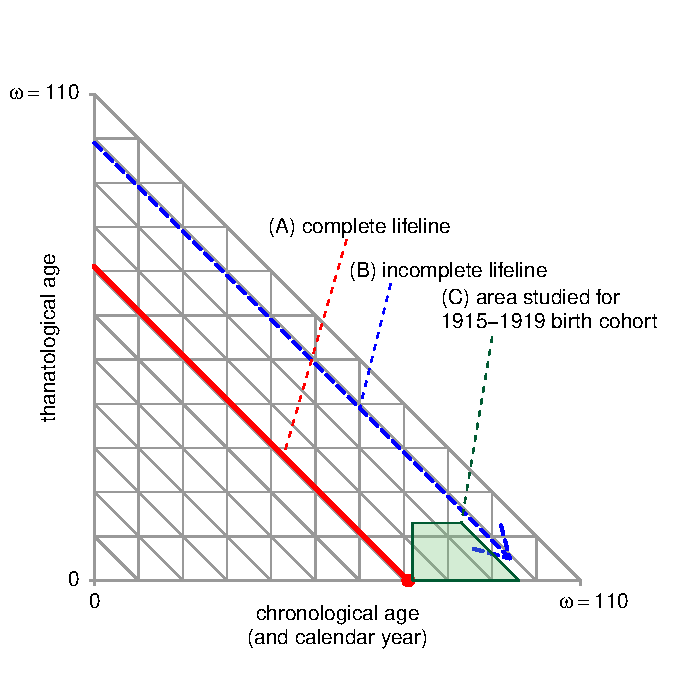
\includegraphics{Figures/LexisOrtho.pdf}
\end{figure}

Underpinning this investigation are a series of demographic surfaces indicating
the average intensity of a given marker along the chronological and thanatological
time dimensions within a series of quinquennial birth cohorts, from which we
focus only on the central 1915-1919 birth cohort.
This visual tool is similar to but orthogonal to the familiar Lexis surface.
Figure~\ref{fig:LexisOrtho} orients the reader with the temporal coordinates we
use. This diagram represents the various possible lifespans within a given birth cohort, with an arbitrary final age, $\omega$, of 110. One's
thanatological age at birth is equal to one's chronological age at death, such
that both axes close out with $\omega$. Members of the birth cohort are born on
the left side of the diagram, at chronological age zero and with an unknown $y$ coordinate (remaining lifetime) at the time of birth.
Lifelines advance downward and to the right, where the downward direction indicates the approach to death, and the
rightward direction represents both the progression of calendar years and
chronological age. The blue arrow (B) indicates a hypothetical lifeline that
will eventually expire at age 99, although this property is unknown until death. The
present study contains only complete lifelines, such as that depicted in the
color red (A) in Figure~\ref{fig:LexisOrtho}, which completes its lifespan at
age 71. In this diagram, diagonal lines represent death cohorts, rather than the
birth cohorts found in the standard Lexis diagram.

We limit the current study to the 1915-1919 cohort due
to the characteristics of the data source. Using the HRS, enough
observations are available such that we can measure the patterns of
within the area outlined in green (C) in Figure~\ref{fig:LexisOrtho}. The
left bound of this area is chronological age 72, and the diagonal right
bound belongs to the completed lifespan of 95. While there are some observations
at thanatological ages greater than 12, there are too few to produce reliable
estimates.\footnote{Since the HRS spans 20 calendar years (1992-2011), the
theoretical upper bound of observation for thanatological age is 20.} Future
waves will expand the area applicable to all but the oldest birth cohorts that are already extinct in the data.

The 1915-1919 birth cohort was exposed to the 1918 Spanish influenza
epidemic as toddlers (1915-1917 cohorts), as infants (1917-1918) cohort and
in-utero (1919 cohort). There is some evidence that this exposure manifested in
various ways in late life \citep[e.g.,][]{almond20061918}, and so the reader may
rightly question whether the results presented here are in some way anomalous.
While more precise methods may detect effects, the methods we expound here are
not precise. Specifically, the smoothing procedure we apply borrows
information from adjacent birth cohorts, which itself may erase whatever
otherwise detectable health artifacts this cohort may have carried into late
life. At these ages, we assume that other risk factors, some of them cumulative
over the life course, senescence itself and other forces likely drive patterns
to a much greater extent. Our justification is here speculative, but we report
that the results for this cohort do not appear visually distinct from those
present in other cohorts. More importantly, our goal here is not to describe the
end-of-life experience of this birth cohort, but to add resolution to the
measurement and description of ageing and morbidity indicators, and contribute
to the practice of demography in general.

\paragraph*{Age}
Thanatological age is calculated for each individual as the lag between
interview and death dates expressed as decimal years. Chronological age is
calculated as the lag between birth and interview date in decimal years. Each
individual is therefore assigned a chronological and thanatological age at each
interview, along with measures of our variables of interest. Since
we are interested in viewing characteristics over both chronological age and
thanatological age simultaneously, we require observations spread over a wide
range of combinations of thanatological and chronological age.

The current HRS dataset runs from 1992 to 2011, which
means that each birth cohort is observed over a different range of ages. For
example, the 1925-1929 cohort enters observation in 1992 at age 62 (at the
youngest) and acheives a maximum completed age of 85 by the end of 2011. On the
other end, the 1905-1909 enters the HRS in 1992 at age 72 at the youngest and
has a maximum completed lifespan of 105 by the last wave in 2011, albeit with
few observations at the upper extreme. Results from these and other birth cohorts are also
valid, but portions of these surfaces are based on fewer data points (lifespans $>$ 100) or ages in which labor market
exits appear to drive patterns at least as much as senescence (ages $<$ 67,
approximately). We selected the 1915-1919 cohort because
its observation window is centered on the chronological ages in which most
deaths occur and in which most recent mortality improvements in
low-mortality countries have occurred ,\footnote{Own calculations based on UN
data \citep{UN2012prospects}. The modal ages at death for the 1915-1919 cohort
are 80-81 for males and around 87 for females. These calculations are based on
partially observed cohort mortality rates, $M(x)$ \citep{HMD}.} and because the
HRS provides a good density and spread of data points over this window. The lower and upper age bounds may vary if questions were not available in the first, second or final waves.

\paragraph*{Characteristics}
We aim for a broad overview of the age variation across different dimensions of
old-age disability and wellbeing. For this reason we select a wide variety of
questions from the HRS data. These include questions
grouped roughly into the following categories: 

\begin{enumerate}
  \item Activities of Daily Living (ADL): six items, and two composite indices.
  \item Instrumental Activities of Daily Living (IADL): seven items and two
  composite indices.
  \item Health Behaviors: five items.
  \item Functional Limitations: six items.
  \item Chronic Conditions: eight items and one composite index.
  \item Cognitive Function: 15 items and two composite indices.
  \item Psychological Wellbeing: nine items and one composite index.
  \item Healthcare Utilization: 14 items.
\end{enumerate}

The the specific variables included in our survey are found in the appendix
tables following the same numbering scheme as above. In all, we summarize
results from 78 individual and composite items.
We excluded variables that were not asked continuously from at least wave 3 through 9. Variables not available in the
first or second wave have left age bounds at higher ages than 72, whereas items
not asked in wave ten have upper lifespan bounds that are below 95.

Each survey question must be in a format suitable for numeric operations.
This requires some compromises in data quality, since some coded responses are less directly
quantifiable, and our translation of categorical or ordinal responses to numeric
values was at times improvised. In most cases, responses are easy to imagine as
``good'' and ``bad'', in which case we assigned higher values to ``bad'' and
lower values to ``good'' outcomes. For example, respondents were asked if they
felt depressed. We assigned 0 to answers of ``no'' and 1 to answers of ``yes''.
Rather than divide all questions into binary responses, we assigned intermediate
values on a case by case basis. For example, self-reported health
had possible responses of ``excellent'', ``very good'', ``good'',
``fair'', and ``poor'', which we assigned values in equal intervals
from 0 to 1, respectively. Some response
sets for particular questionnaire items changed between
waves.
In these cases, we attempted to assign numerical codes that were consistent
over the transition. These recodes are imprecise, but they are good enough
to meet the goals of this study. In other words, the surfaces we
present are not exact measurements, but are meant to provide
\textit{impressions} about how characteristics change over age.\footnote{The
pre-processing of variables is full of details that would clutter this paper.
Rather than a lengthy and detailed appendix describing the case by case
treatment of variables, we make the full code base used in the generation of
results available in an open repository.}

Variables with compact or bounded numeric responses were rescaled to range from
0 to 1. Variables with no clear bounds or very large upper
bounds, such as medical expenditure, body mass index, or number of hospital
visits were not rescaled. These rescalings are intended to simplify
the visual interpretation of surfaces, and they do not alter the
quantitative summary measures we use later. 

Some questionnaire items in the HRS are only asked every second interview. In
these cases, we impute within-individual trajectories assuming a linear
trend. For example one item asks respondents whether they experience back
pain. If in wave 3 an individual responded ``no'', wave 4 is skipped, and in
wave 5 the respondent answered ``yes'', then we assign 0 to wave 3, 0.5 to wave
4 and 1 to wave 5 for this question. If a response is missing in a given wave,
but available in the previous wave, we carry it over as a constant, but we do
not impute backwards in time. We also do not impute questions that were not part
of the questionnaire for a given wave. These within-individual procedures reduce
missing cases for within valid interviews by 30-40\%, which in some cases provides our statistical
procedures with a better fit, but does not skew results.
% TODO continue here

\paragraph*{Weighting}
The population universe of the HRS and this study is the resident
population of the United States. Therefore person weights are needed in
order to estimate population-level means. 
One difficulty with the HRS is that the institutionalized population is treated
as a second target population. In all waves but 5 and 6, there are no person weights
assigned to institutionalized individuals. We try to impute missing
person-weights according to some simple assumptions. If the individual was
assigned a weight in a previous wave, we carry this weight over as a constant, unless there was also a non-zero weight in a future interview, in
which case we assign the weight according to the within-individual linear
pattern. Individuals and interviews that still have missing person-weights
after this procedure are discarded from our study. Person weights compensate for
minor detectable attrition in the HRS \citep{kapteyn2006effects}, which for
our purposes may be considered unbiased \footnote{Small biases in the survey
only appear with respect to baseline characteristics that we do not consider.
Attrition due to health conditions, e.g., mental impairment, is mostly mitigated
due to the use of proxy respondents in such situations \citep{weir2011proxy}.}.

\paragraph*{Loess smoothing}
Direct tabulations of the weighted data are legible if all birth
cohorts are combined, but doing this distorts results due to cohort
composition bias. To overcome birth cohort heterogeneity within surfaces,
we use birth cohorts as a third time dimension. Tabulations within this three dimensional space are noisy, and so we
enhance surface legibility by using a non-parametric local smoother.
We specify a loess model of the given characteristic over chronological age,
thanatological age, and quinquennial birth cohorts, using all observations of since-deceased individuals from the 1900 through the 1934 birth cohorts. We fit the model using the \texttt{loess()} function in base \texttt{R} \citep{cleveland1992local,Rcore2013}\footnote{Using the fitted model, surfaces are produced using the related loess prediction function, \texttt{predict.loess()}. The smoothing parameter, \texttt{spar}, is set to 0.7 for the results we present in the paper.
All results were also produced using smoothing parameters of .5, and .9, and
we concluded that the specific choice of smoothness does not drive results.
The three predictor dimensions are not normalized, in order to preserve year
units. } to the weighted individual-level data for each sex separately, and then
predict a surface for the 1915-1919 birth cohort within the study area outlined
in green (C) in Figure~\ref{fig:LexisOrtho}. Weighting is therefore explicit by
person-weights, and implicit by point density within the three temporal
dimensions.\footnote{Note that smoothing over these three particular time dimensions is not an
overidentification. Within a cohort, to smooth over thanatological age,
chronological age and completed lifespan would be an overidentification, similar
to the familiar APC problem. The full set of lifespan indices the
demographer has to choose from are: birth cohort, death cohort,
chronological age, thanatological age, complete lifespan, and period. Within
this set of six lifespan dimensions, some combinations invoke overidentification
and others do not. For instance, it would be possible to smooth over years
lived, years left, and period in this case, but birth cohorts are the more
meaningful category for this study.}

\section*{Results}

We first present examples of four surfaces that exemplify the major ways in
which characteristics tend to vary temporally over the lifespan within a birth
cohort. These four major patterns of variation provide a way to categorize and
understand markers of ageing. We summarize the results of our set of 78
characteristics by calculating Pearson correlation coefficients for each of
these four axes and display results graphically, as well as in an appendix
table.

\paragraph{Four major surface axes}
In most situations it is obvious to the eye whether a
variable operates over thanatological age or over chronological age, but there
are many instances where both are at play, or where the relationship is
complex. We first present surfaces representing psychological problems for males
(Figure~\ref{fig:psych}) and back pain for females (Figure~\ref{fig:back}).
These two surfaces are examples of thanatological and
chronological characteristics, respectively.

From the direction of the contours on the surface in Figure~\ref{fig:psych}, we
conclude that the chances of ever having been diagnosed with psychological
problems increases with the approach to death and not with the advancing of
chronological age, at least in the window of observation studied here.
However, since the risk of death itself also increases according to an
exponential pattern in these same ages, aggregating individual results by
chronological age produces an increasing pattern over age for this same
characteristic (see Figure~\ref{fig:chronofalse}).
In this case, the apparent chronological age pattern is due
to an interaction between the thanatological pattern seen in
Figure~\ref{fig:psych} and the age pattern of mortality itself. We argue that it
is imprecise to consider chronological age a risk factor for characteristics that display such strong thanatological patterns, as an
apparent chronological age pattern along said margin is a deceptive artifact.
Instead, such characteristics appear to more closely operate as effects of the body shutting down or possibly as a signal on average that death is not far off, a demographic corroboration of substantive findings in the psychology literature \citep{carstensen2006influence}. Many characteristics studied here display patterns that are strongly thanatological.

Figure~\ref{fig:back} tells just the opposite story about back pain for females.
Back pain is a function of
chronological age, at least at the population level until around chronological
age 90. This is the dominant way of thinking about most aspects of the ageing
process. In these ages, back problems provide no information about remaining
years of life. Of the characteristics included in this
study, only current smoking, arthritis, and self reports of current versus former memory exhibit such clear chronological patterns (both for males and
females).
\begin{figure}[!h]
 \centering
   \caption{Psychological problems (ever) by chronological age only. Males, 1915-1919 birth
    cohort. With 95{\%} confidence bands from loess fit.}
    \label{fig:chronofalse}
   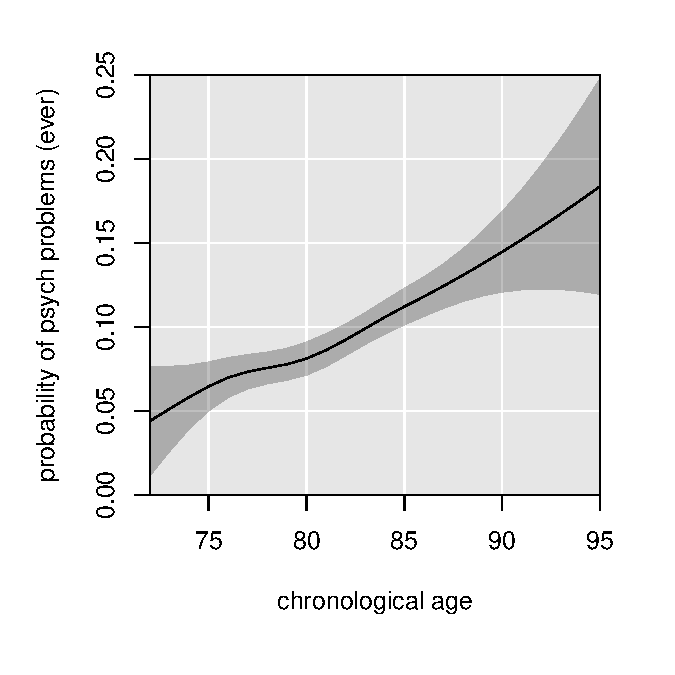
\includegraphics[scale=.7]{Figures/MalePsychChrono.pdf}
\end{figure}

\begin{figure}[!h]
    % This figure was produced in
    % \makebox[\textwidth][c]{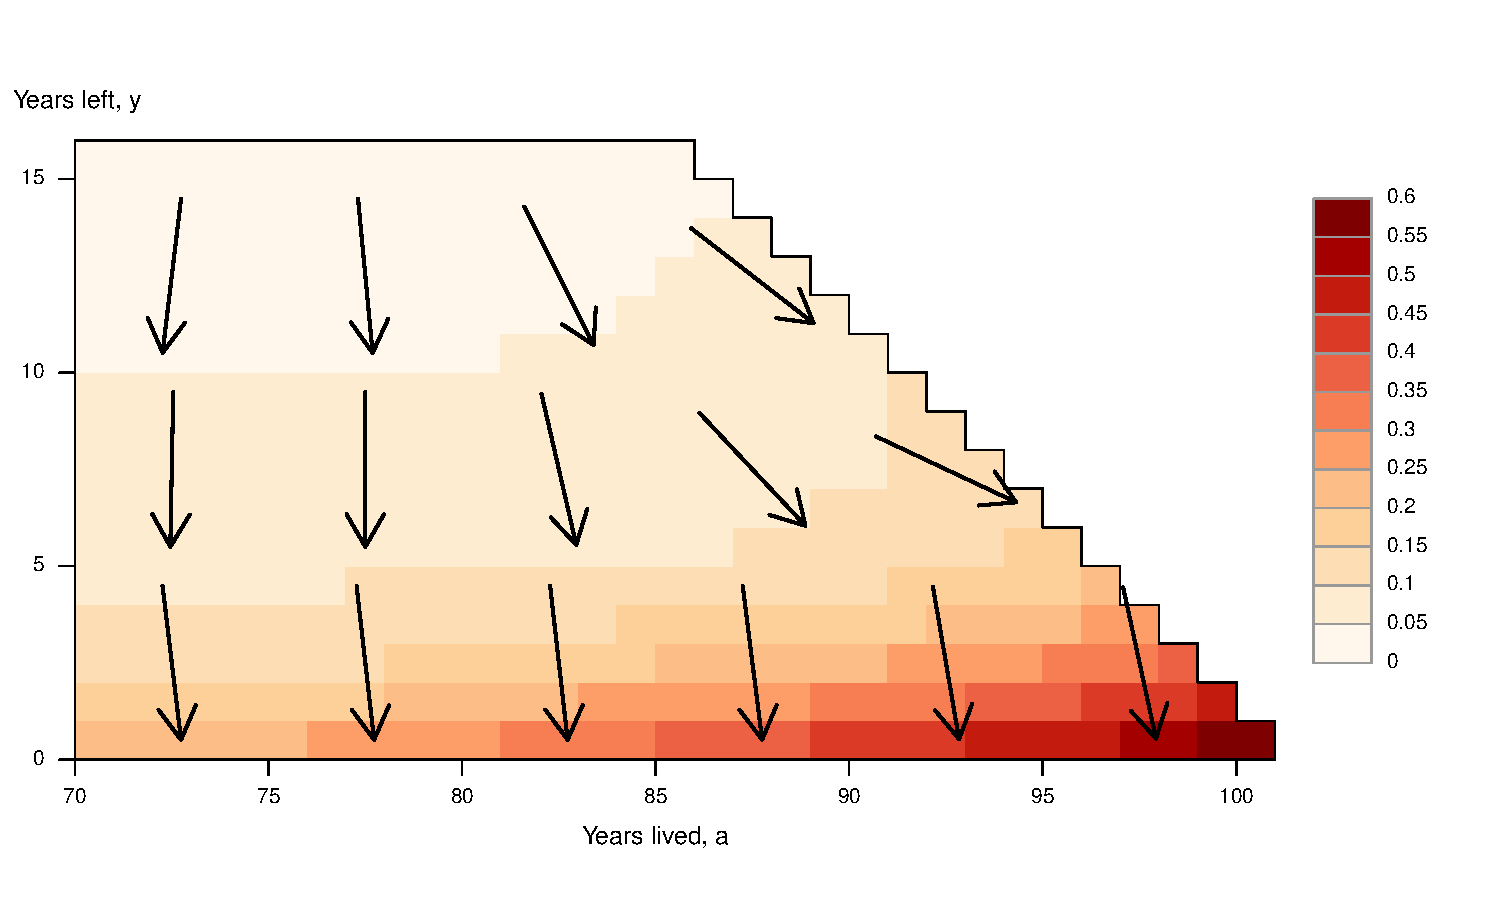
\includegraphics[scale=.6]{Figures/SurfExampleMalesSRH.pdf}}
    \centering
    \caption{Examples of characteristics that vary along the thanatological and
    chronological age axes.}
    \label{fig:thanochrono}
    \begin{subfigure}{\linewidth}
    \caption{Psychological problems (ever) by
    years lived (x axis) and years left (y axis). Males, 1915-1919 birth cohort.
    }
    \label{fig:psych}
	\vspace{-2em}
	\makebox[\textwidth][c]{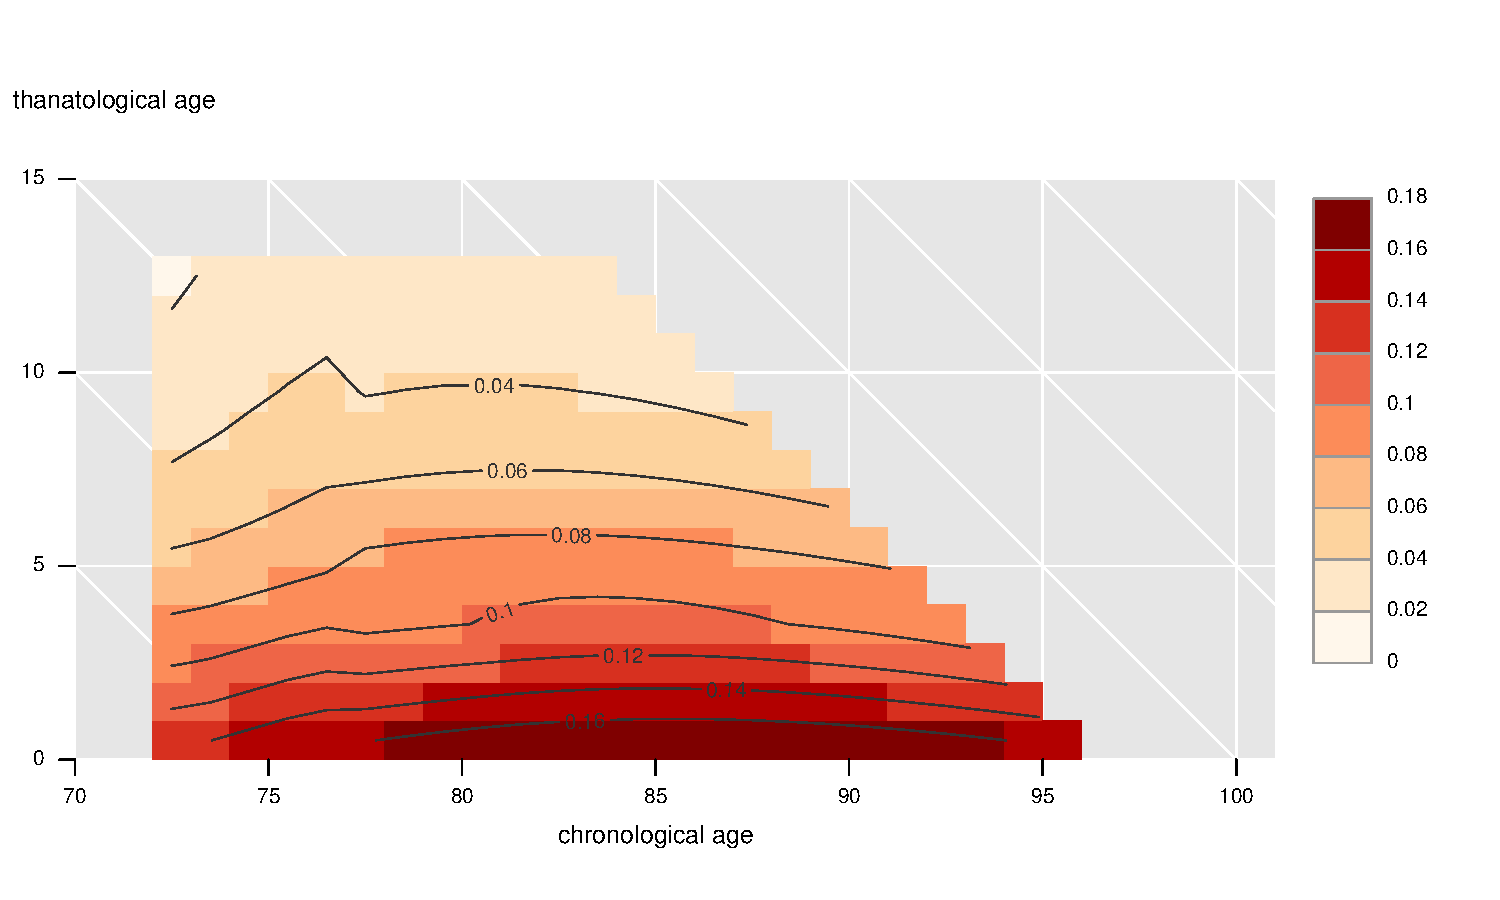
\includegraphics[scale=.6]{Figures/Surf_Male_psych.pdf}}
	\end{subfigure}
	
	\begin{subfigure}{\linewidth}
    \caption{Back Problems by
    years lived (x axis) and years left (y axis). Females, 1915-1919 birth
    cohort.}
    \label{fig:back}
	\vspace{-2em}
	\makebox[\textwidth][c]{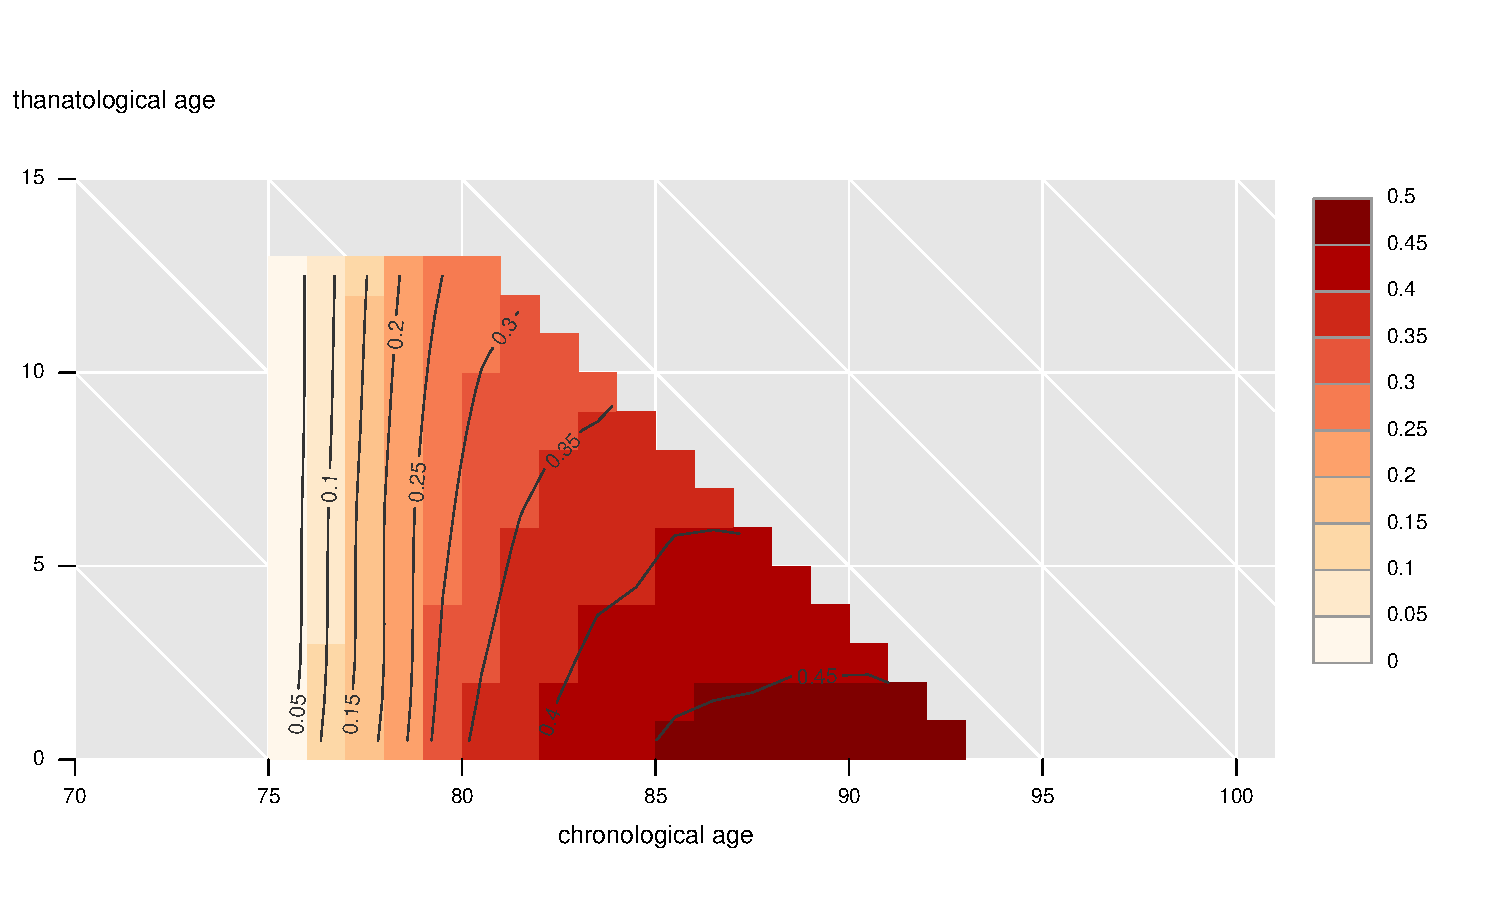
\includegraphics[scale=.6]{Figures/Surf_Female_back.pdf}}
	\end{subfigure}
\end{figure}
\FloatBarrier

Other informative patterns also exist among the set of characteristics studied.
These include characteristics that vary by lifespan. Characteristics that vary
by lifespan appear constant within lifespans. These are often characteristics that
\textit{determine} lifespan. Ever smoking displays such a pattern, as seen in
Figure~\ref{fig:evsmkng} for females of the 1915-1919 cohort. This pattern is
also a corroboration of science and common sense: smoking kills (at least in
this range of lifespans). Other variables that display similar patterns in this
window of the lifespan include lung disease among males (this is largely
redundant with the former), dental visits in the previous year (both sexes),
and diabetes among females. Sometimes such patterns combine in complex ways
worthy of further study.

The fourth major axis of contour variation runs perpendicular to lifelines. One
characteristic that clearly displays this pattern is ever having been
diagnosed with high blood pressure among males. This characteristic varies by
lifespan, and thanatological age within lifespan within the window of study.
In other words, longer lifespans display later onset but greater eventual odds of
having been diagnosed with high blood pressure. Arithmetically, $years~lived - years~left$ is the
operative predictor of blood pressure. For example, for
such characteristics, the condition of a 70-year old with five
remaining years of life may resemble that of an 80-year old with
15 remaining years of life. Such characteristics are not very useful alone for
predicting eventual lifespan.\footnote{We do not have expertise to comment further on blood pressure, but instead only provide an interpretation of the surface presented.} Contours such as this imply that variation for a characteristic

\begin{figure}[!h]
    % This figure was produced in
    % \makebox[\textwidth][c]{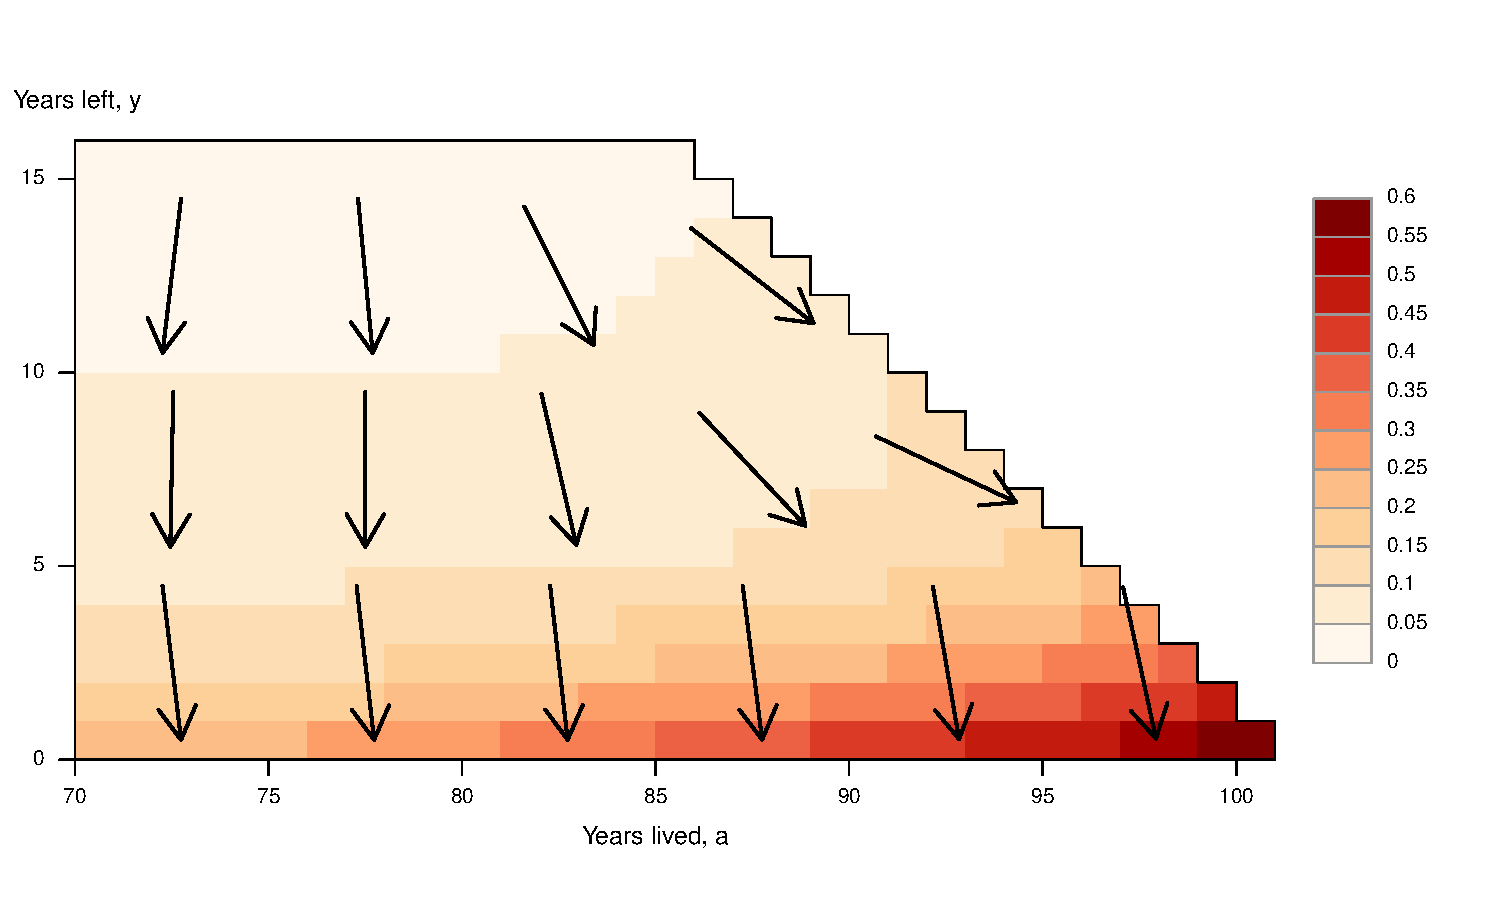
\includegraphics[scale=.6]{Figures/SurfExampleMalesSRH.pdf}}
    \centering
    \caption{Examples of characteristics that vary by lifespan only or by
    thanatological age within lifespan.}
    \label{fig:lifespan}
    \begin{subfigure}{\linewidth}
    \caption{Smoking (ever) by
    years lived (x axis) and years left (y axis). Females, 1915-1919 birth
    cohort.
    }
    \label{fig:evsmkng}
	\vspace{-2em}
	\makebox[\textwidth][c]{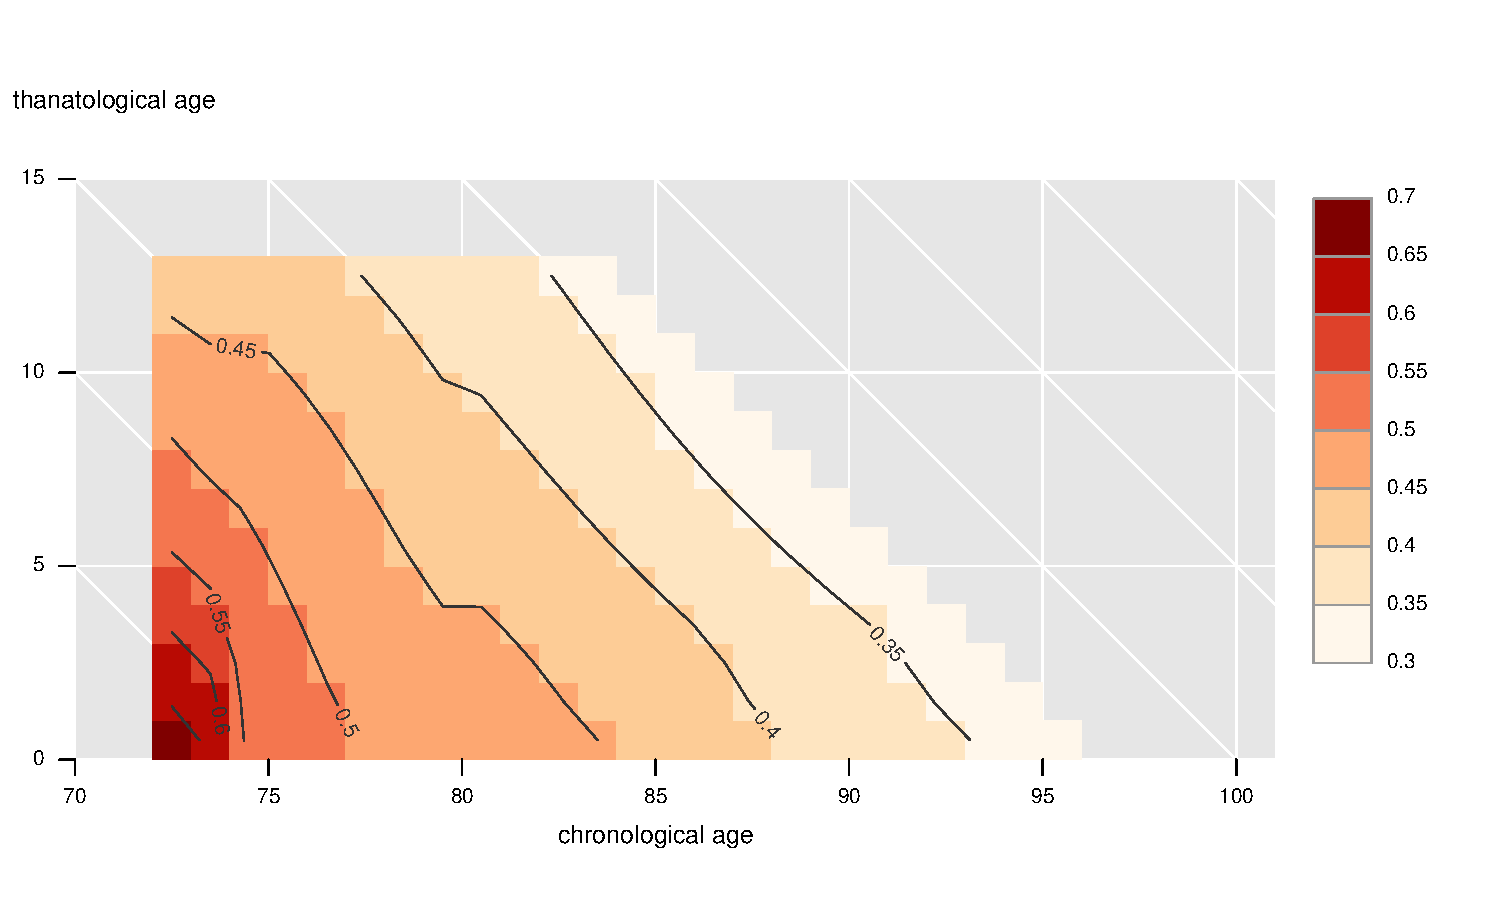
\includegraphics[scale=.6]{Figures/Surf_Female_smoke_ev.pdf}}
	\end{subfigure}
	
	\begin{subfigure}{\linewidth}
    \caption{Blood Pressure by
    years lived (x axis) and years left (y axis). Males, 1915-1919 birth
    cohort.}
    \label{fig:bp}
	\vspace{-2em}
	\makebox[\textwidth][c]{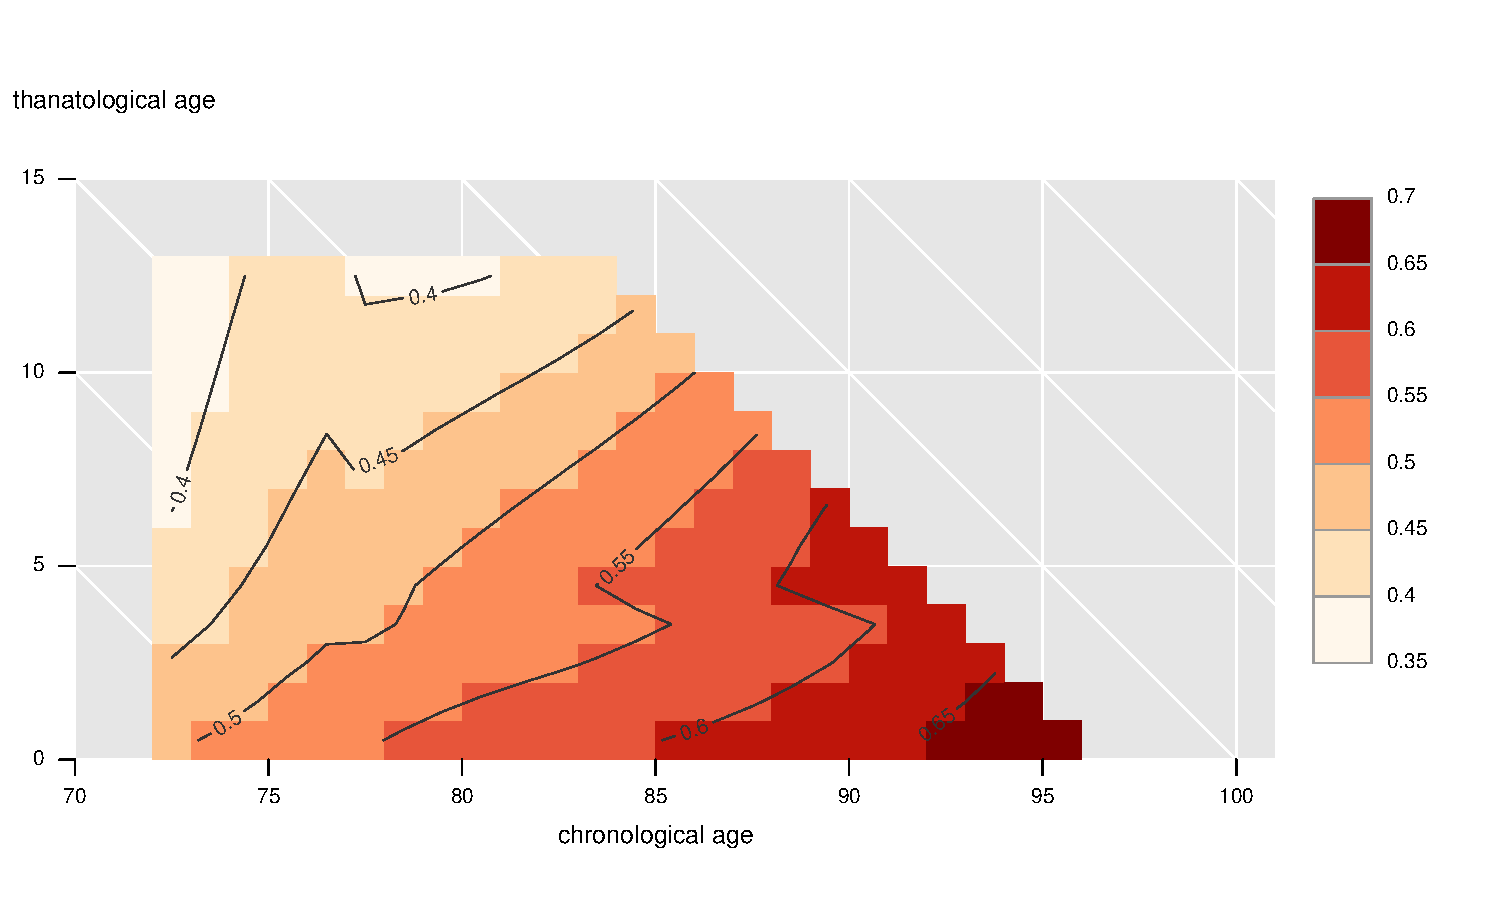
\includegraphics[scale=.6]{Figures/Surf_Male_bp.pdf}}
	\end{subfigure}
\end{figure}
\FloatBarrier

\paragraph{Summary of results for all characteristics}
Surfaces such as those in Figures~\ref{fig:thanochrono} and~\ref{fig:lifespan}
were produced for all 78 variables and each sex. We distill these surfaces into
four Pearson correlation coefficients, each designed to capture the variation along one of the axes explained above. We call the four axes
thanatological, chronological, lifespan ($chrono+thano$), and mixed
($chrono-thano$). For a given surface, we calculate the correlation
coefficient of the matrix elements against the four margin indices one at a
time (rather than using the survey microdata).
Most characteristics are summarized nicely by either one or two of these axes.
We display these correlation coefficients by juxtaposing perpendicular axes in
scatter plots separately for males and females.

\begin{figure}[!h]
    % This figure was produced in
    % \makebox[\textwidth][c]{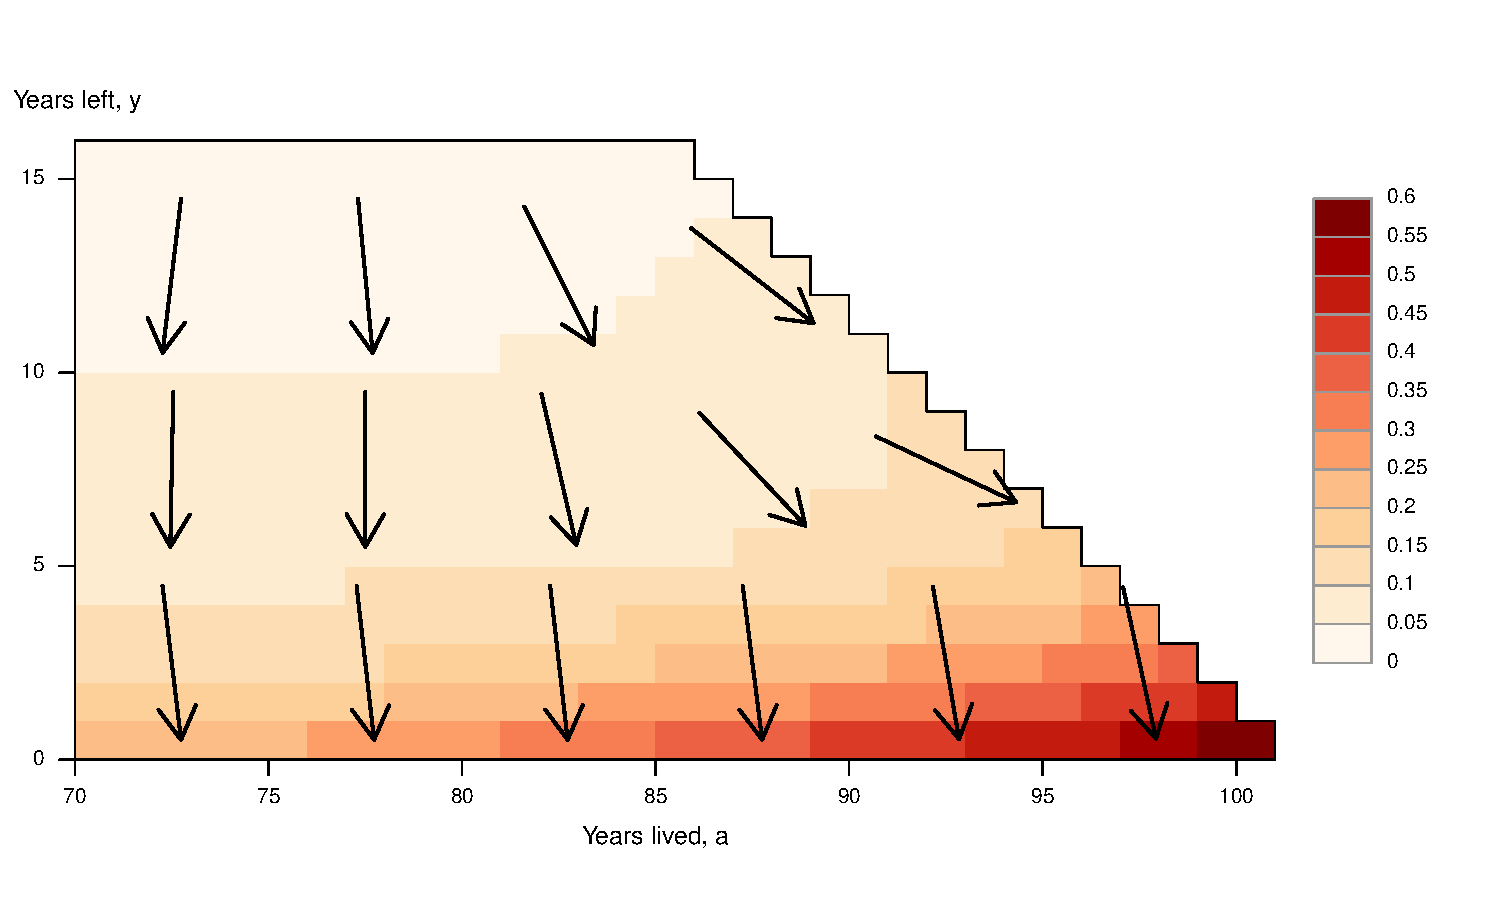
\includegraphics[scale=.6]{Figures/SurfExampleMalesSRH.pdf}}
    \centering
    \caption{Thanatological versus chronological correlation, with selected
    characteristics labeled. 1915-1919 birth cohort, chronological ages 72-95.}
    \label{fig:thanochronocorr}
    \makebox[\linewidth][c]{
    \begin{subfigure}{0.7\textwidth}
    \caption{Males}
    \label{fig:malcorr1}
	\vspace{-2em}
	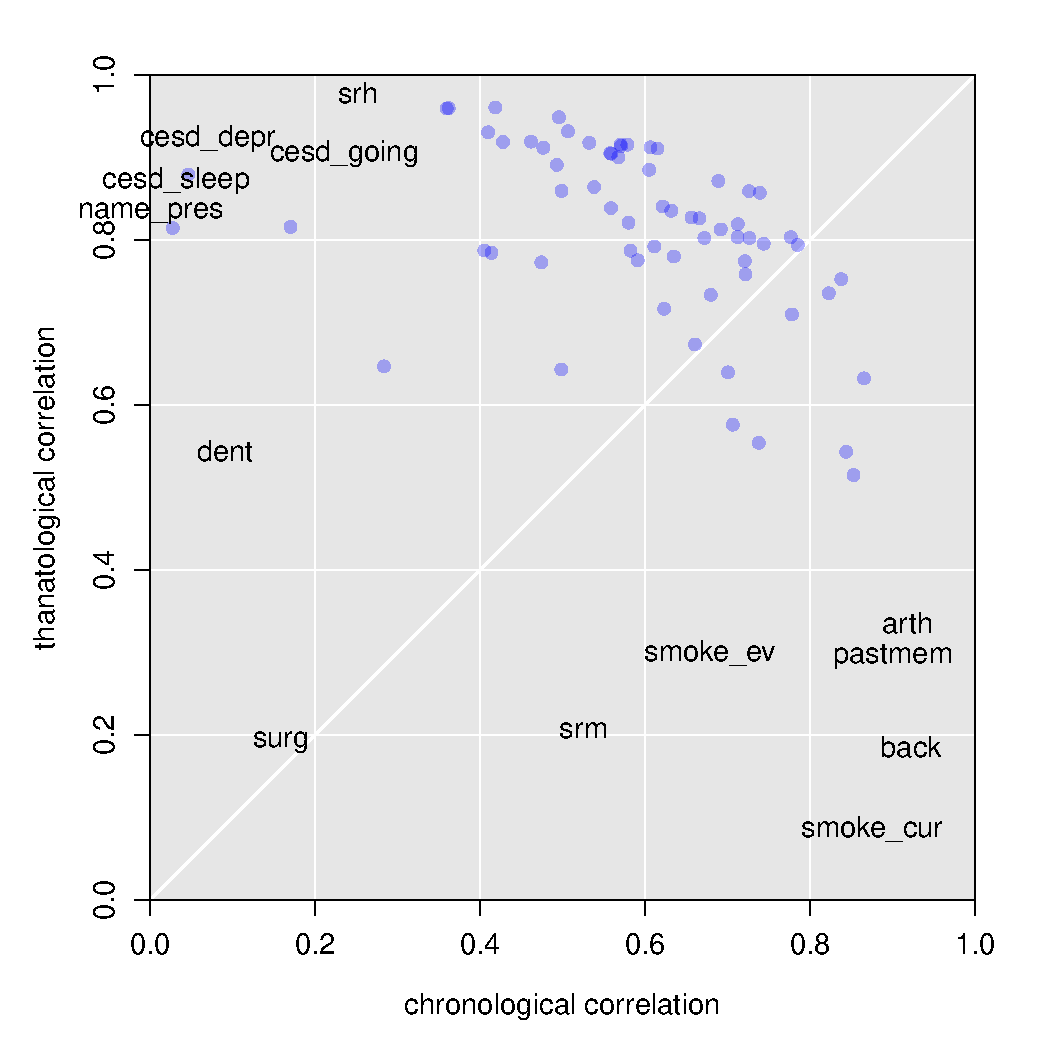
\includegraphics[width=.95\textwidth]{Figures/MaleCorr1.pdf}
	\end{subfigure}
	\hspace{-1em}
	\begin{subfigure}{.7\textwidth}
    \caption{Females}
    \label{fig:femcorr1}
	\vspace{-2em}
	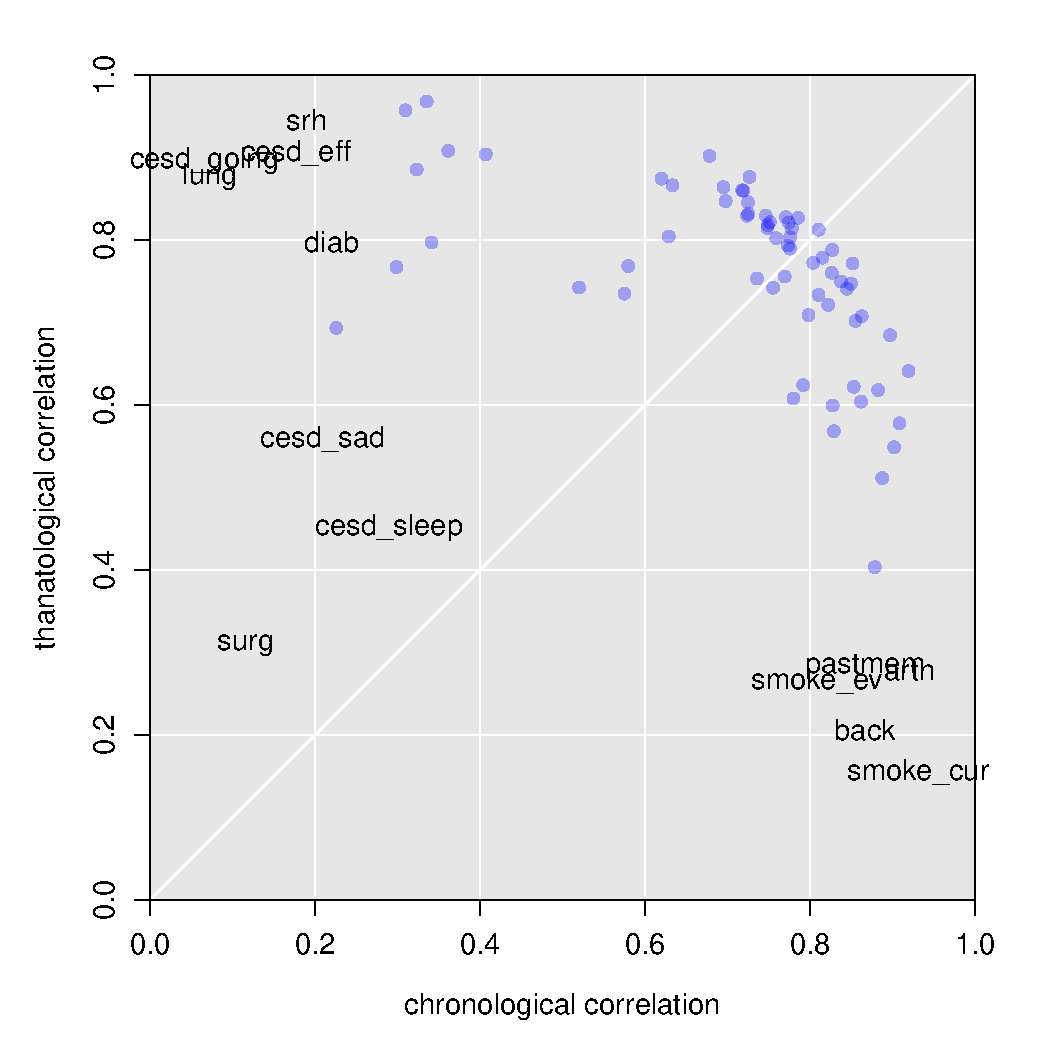
\includegraphics[width=.95\textwidth]{Figures/FemaleCorr1.pdf}
	\end{subfigure}
	}
\end{figure}
	
Figure~\ref{fig:thanochronocorr} displays the simple correlation coefficients
that belong to the chronological and thanatological axes. For males, 45
variables display thanatological correlations of greater than 0.8, versus nine chronological
correlations above the same threshold. For females, the figures are 32 and 29,
respectively, a different picture overall. Both point clouds are in high
thanatological ages, but females lean further towards chronological variation
within this cohort. That thanatological patterns are somewhat less accentuated for females may
corroborate aspects of the existing literature on sex differences in morbidity and mortality \citep{case2005sex}.
	
\begin{figure}[!h]
    % This figure was produced in
    % \makebox[\textwidth][c]{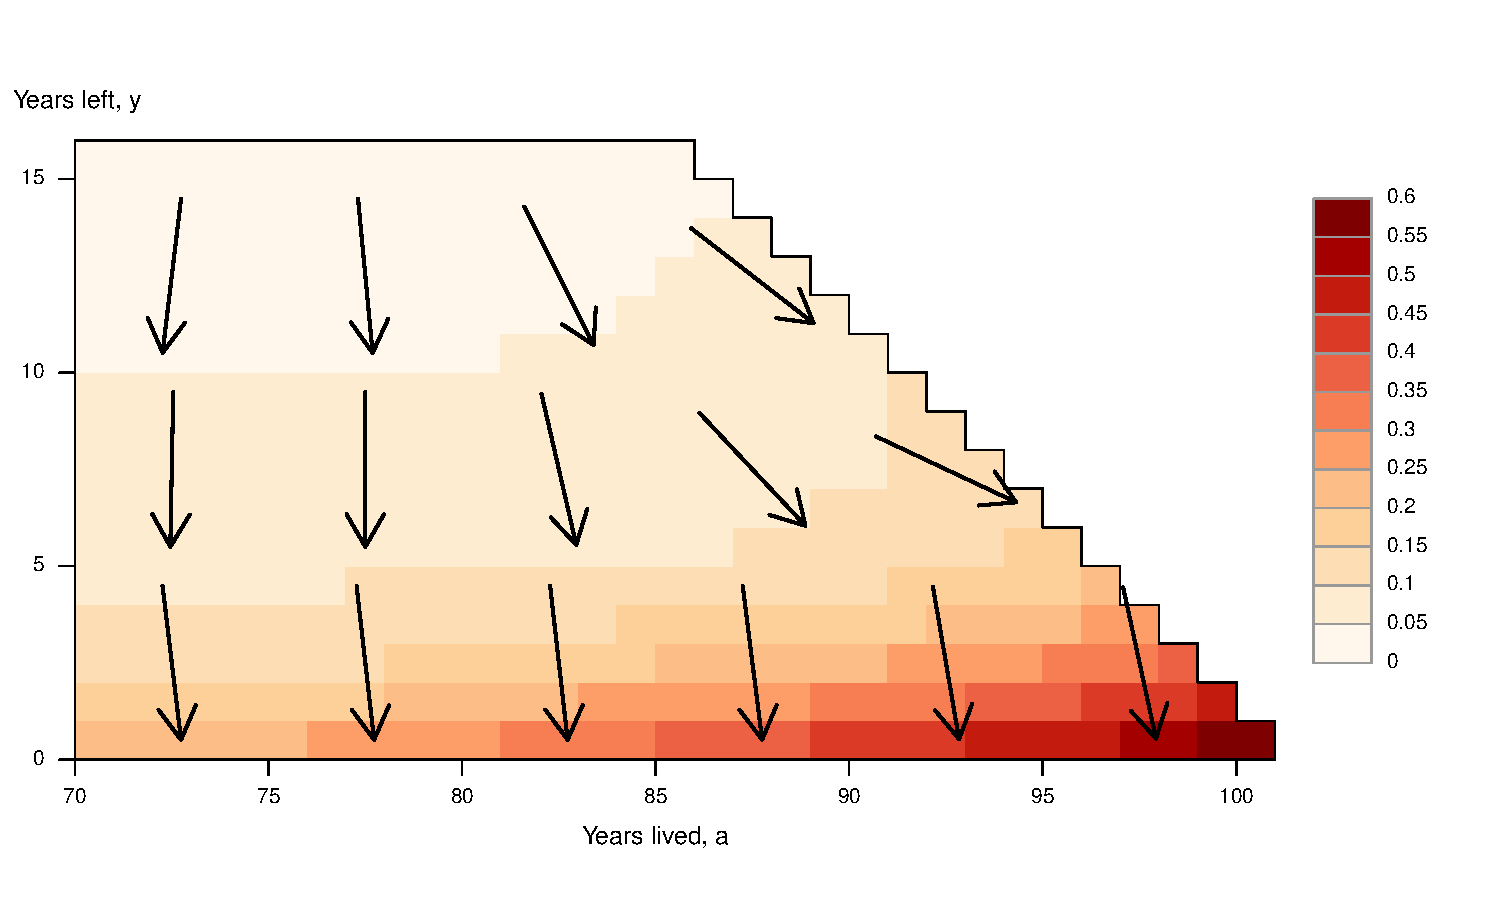
\includegraphics[scale=.6]{Figures/SurfExampleMalesSRH.pdf}}
    \centering
    \caption{Lifespan versus mixed correlation, with selected
    characteristics labeled. 1915-1919 birth cohort, chronological ages 72-95.}
    \label{fig:lifespanmixed}
	    \makebox[\linewidth][c]{
    \begin{subfigure}{0.7\textwidth}
    \caption{Males}
    \label{fig:malcorr2}
	\vspace{-2em}
	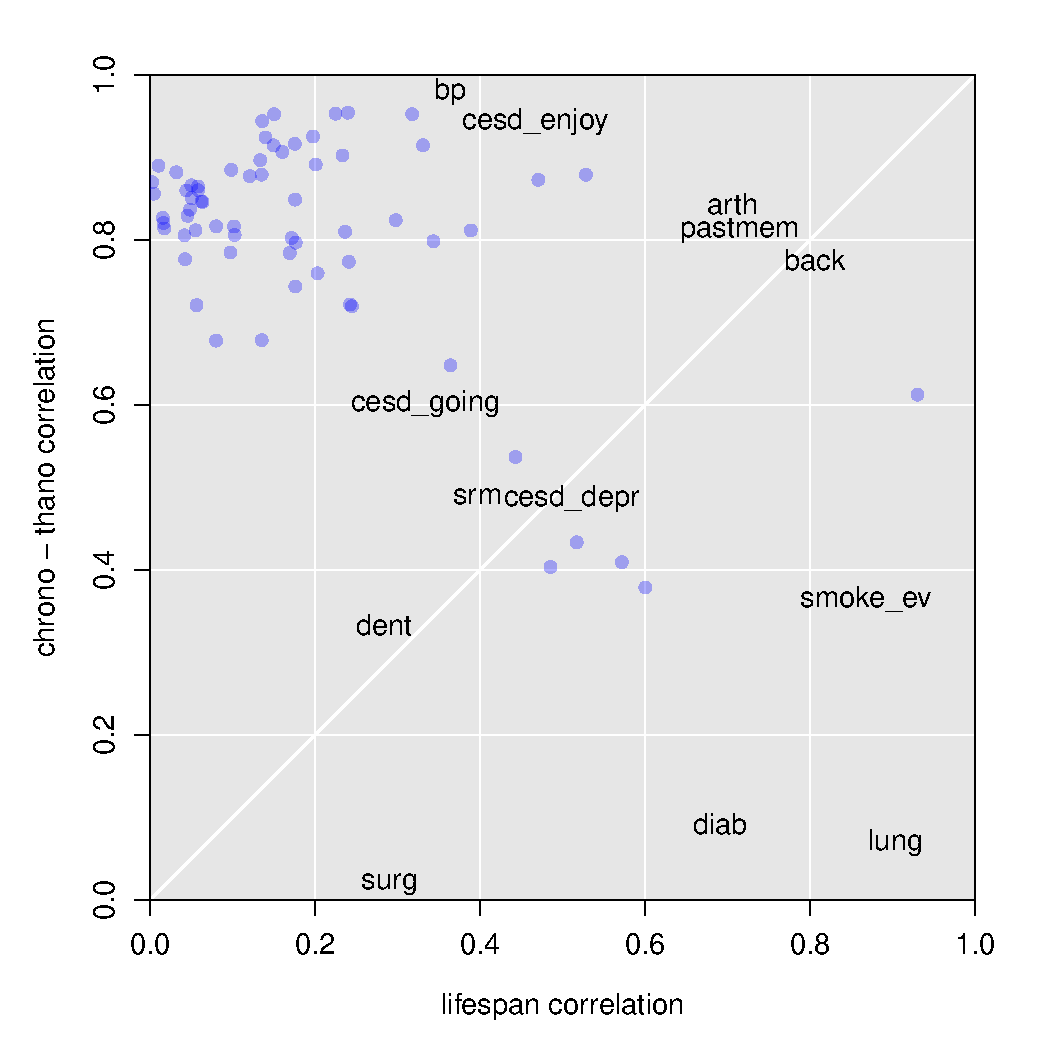
\includegraphics[width=.95\textwidth]{Figures/MaleCorr2.pdf}
	\end{subfigure}
	\hspace{-1em}
	\begin{subfigure}{.7\textwidth}
    \caption{Females}
    \label{fig:femcorr2}
	\vspace{-2em}
	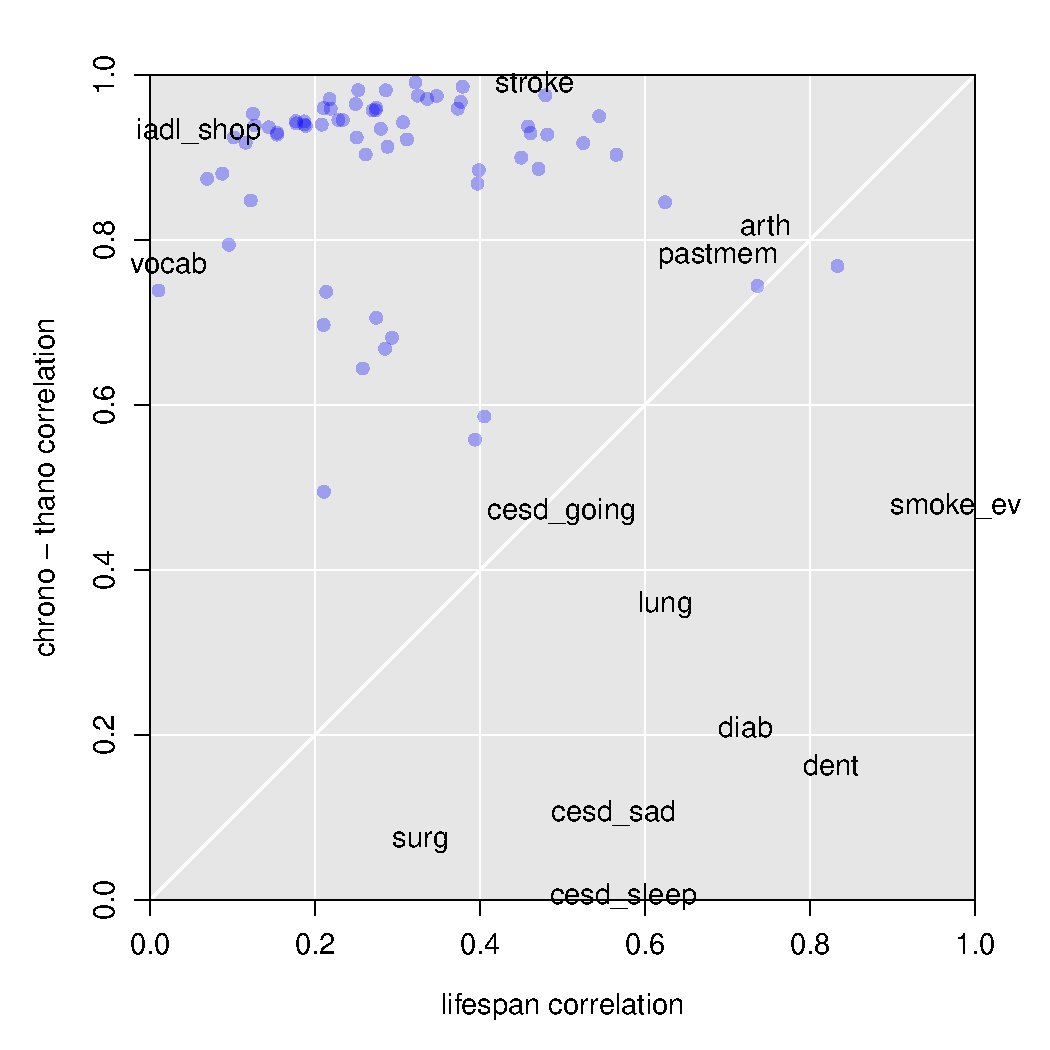
\includegraphics[width=.95\textwidth]{Figures/FemaleCorr2.pdf}
	\end{subfigure}
	}
	
\end{figure}

Figure~\ref{fig:lifespanmixed} displays correlation coefficients
that belong to the lifespan and ``mixed'' axes. Among males, four variables
display lifespan correlations of greater than 0.8, versus 49 mixed correlations above
the same threshold. For females, the respective figures are three and 55. The
mixed axis ($chrono age - thano age$) is the winner among the set of
characteristics tested. The appendix provides detailed results. 

\section*{Discussion}
The distribution of tested characteristics with respect to the
four axis orientations described here is striking. However, these findings
must be tempered by noting that 1) the summary measure (correlation coefficient)
used here blends out some information, 2) these results may
not necessarily extrapolate to the set of all testable questions in the HRS, and 3) this relationship does not necessarily hold in other windows of the lifespan or other birth cohorts. Further, the patterns
presented here are valid for the whole population (of a given sex) taken
together, but were the target population split by causes of death (for
instance), the patterns may change. For example, imagine hypothetically that the
strong thanatological pattern shown in Figure~\ref{fig:thanochrono}
(psychological problems) were driven by strong patterns within individuals that
eventually die of suicide, but that other causes of death displayed entirely different patterns with respect to
psychological problems. Such cases are easily imaginable for other
characteristics and causes of death. At the time of this research, we did not
have access to cause of death information from the HRS mortality followup. For
detailed investigations of particular characteristics, cause-conditioning
surfaces would clearly aid in disentangling morbidity processes.

Research to better document the multidimensional age variation of particular
characteristics would benefit from more careful measurement than that conducted
here.
Despite such shortcomings, the principle aim of this study has been satisfied:
this survey of characteristics highlights the complex variety of age and
lifespan dimensions over which some key aspects of the aging process unfold. All
of the indicators we tested are commonly used to describe population ageing, and
very few of them are exclusively a function of chronological age. If this
finding is sustained in other cohorts and populations, and if other indicators
here untested also display similar temporal complexity, we submit that the
common discourse and debate on the nature and impacts of ageing ought to be
better informed by more judicious measurement and description in terms of
thanatological and chronological age.

We hope that the conceptual model of the
lifespan presented here, which complements the Lexis diagram, will be of use to
demographers. Other combinations of lifespan time dimensions are also possible,
and these would highlight different patterns in data. The variety and
availability of such options, perhaps now placed in starker relief, demands a more nuanced
understanding of the temporal accounting that relates demographic time
perspectives. Further exploration and experimentation with these formal
demographic concepts will lead to a more judicious toolkit for demographic
measurement and the practice of demography, and ultimately a wiser contribution
to the discourse on population ageing. A series of direct applications and
implications derive from the concepts and results presented in this paper. 

First, if
compared between two timepoints, demographic work such as this will
provide a more precise answer to the question or morbidity compression. Given the chronological age ruse exemplified in the case of psychological problems (see Figures~\ref{fig:chronofalse} versus~\ref{fig:psych}), it is safe to say that unless retrospective
thanatological measurements of morbidity dimensions are undertaken, we do
not have direct information about whether compression is (or has
been) happening or not. Using the techniques shown here, the researcher may
directly estimate the varieties of end-of-life profiles often seen in the
literature on morbidity compression \citep[e.g.,][]{fries2011compression}. That
is, changing chronological age patterns may be coincidental.

Second, large scale panel studies may be motivated to
implement, increase, or improve mortality follow-up modules. Information
on the full age dimensions of health outcomes will be valuable. The good news is
that many unlinked panel studies may be linked to death registers in
retrospect. A few populations with long-running and fully linked
population registers already preside over such information, and we encourage a
more thorough exploration of the temporal richness in population change and
population characteristics. Underused as it is, the Lexis surface does not tell
the whole story! 

Third, health care providers and the public may better situate the association
of certain health outcomes with stages of the ageing process. This is both a
question of allocating resources and a question of how individuals conceive of
themselves with respect to age. In this regard, we add to the chorus of
researchers working to change the measurement of age to reflect the changing
experience of age \citep[see e.g.,][]{sanderson2013characteristics}. 

Fourth,
this material highlights important sex differences in the onset and trajectory
of some aspects of morbidity. Some of these differences may
corroborate extant findings, and others may provide new understanding to sexual dimorphism in
morbidity. In general, these methods and measurements are applicable to describe
any between-group disparity in demographic or social outcomes, most of which
directly or indirectly relate to remaining years of life.

We do not, at this time, attempt to thoroughly cluster
characteristics based on the scores of the four different correlation
coefficients, but this may be a fruitful exercise for further work. It is our hope that these results are strongly suggestive and orient
future investigation.

%\FloatBarrier
\singlespacing
\bibliographystyle{plainnat}
  \bibliography{references} 
%  

%\pagebreak
%
\begin{appendices}
\section{Variables and correlations}



\end{appendices}

For tables displayed in this appendix we use a shorthand to identify axis types.
T indicates the correlation coefficient along the thanatological age axis. C
indicates the chronological age axis. $C+T$ indicates the lifespan axis
(right-downward slanting isolines). $C-T$ indicates the mixed axis, the
most common type in this data. Results are available on request as machine
readable data, and the code used to generate these and all other results is
available freely in a repository: 

%(insert url)
\url{https://github.com/timriffe/ThanoEmpirical}

Results are grouped by several major morbidity categories. 

\listoftables

\pagebreak
% ADL
\begin{table}
\small
\begin{adjustwidth}{-5em}{-2em}% 
\centering
\caption{Activities of Daily Living (ADL)}
\label{tab:ADL}
\begin{tabular}{L{4em}
L{3cm}|C{1cm}C{1cm}C{1cm}C{1cm}|C{1cm}C{1cm}C{1cm}C{1cm}}
  \multicolumn{2}{c|}{Variable}&\multicolumn{4}{c|}{Males} &
 \multicolumn{4}{c}{Females} \\
 \midrule
Short & Long & T & C & $C+T$  & $C-T$  & T & C & $C+T$ &
$C-T$ \\
\midrule 
adl3 & ADL 3-point & 0.83 & 0.67 & 0.10 & 0.89 & 0.80 & 0.76 & 0.21 & 0.94 \\ 
   \rowcolor[gray]{.9}adl5 & ADL 5-point & 0.83 & 0.63 & 0.06 & 0.86 & 0.81 & 0.75 & 0.19 & 0.94 \\ 
  adl\_walk & Diff. walking across room  & 0.86 & 0.54 & 0.06 & 0.81 & 0.83 &
  0.72 & 0.15 & 0.93 \\
   \rowcolor[gray]{.9}adl\_dress & Diff. dressing  & 0.82 & 0.71 & 0.15 & 0.92 & 0.82 & 0.75 & 0.19 & 0.94 \\ 
  adl\_bath & Diff. bathing or showering  & 0.84 & 0.62 & 0.04 & 0.86 & 0.82 &
  0.75 & 0.19 & 0.94 \\
   \rowcolor[gray]{.9}adl\_eat & Diff. eating  & 0.80 & 0.67 & 0.12 & 0.88 & 0.76 & 0.77 & 0.25 & 0.92 \\ 
  adl\_bed & Diff. getting in/out bed  & 0.82 & 0.58 & 0.02 & 0.82 & 0.83 & 0.72 & 0.15 & 0.93 \\ 
   \rowcolor[gray]{.9}adl\_toilet & Diff. using toilet & 0.84 & 0.56 & 0.02 & 0.81 & 0.73 & 0.81 & 0.31 & 0.94 \\ 
   \bottomrule
\end{tabular}

  \end{adjustwidth}
  \end{table}
  
% IADL
\begin{table}
\small
\begin{adjustwidth}{-5em}{}% 
\centering
\caption{Instrumental Activities of Daily Living (IADL)}
\begin{tabular}{L{4em}
L{3cm}|C{1cm}C{1cm}C{1cm}C{1cm}|C{1cm}C{1cm}C{1cm}C{1cm}}
  \multicolumn{2}{c|}{Variable}&\multicolumn{4}{c|}{Males} &
 \multicolumn{4}{c}{Females} \\ 
 \midrule
Short & Long & T & C & $C+T$  & $C-T$  & T & C & $C+T$ &
$C-T$ \\
\midrule 
iadl3 & IADL 3-point & 0.89 & 0.60 & 0.00 & 0.87 & 0.77 & 0.80 & 0.27 & 0.96 \\ 
   \rowcolor[gray]{.9}iadl5 & IADL 5-point & 0.90 & 0.57 & 0.05 & 0.85 & 0.83 & 0.75 & 0.18 & 0.94 \\ 
  lim\_work & Health limits work & 0.93 & 0.51 & 0.08 & 0.82 & 0.97 & 0.34 & 0.27 & 0.71 \\ 
   \rowcolor[gray]{.9}iadl\_map & Diff. using map & 0.73 & 0.82 & 0.32 & 0.95 & 0.79 & 0.83 & 0.29 & 0.98 \\ 
  iadl\_tel & Diff. using telephone & 0.80 & 0.78 & 0.23 & 0.95 & 0.70 & 0.85 & 0.37 & 0.96 \\ 
   \rowcolor[gray]{.9}iadl\_money & Diff. managing money & 0.91 & 0.56 & 0.06 & 0.85 & 0.81 & 0.78 & 0.22 & 0.96 \\ 
  iadl\_meds & Diff. taking meds & 0.92 & 0.46 & 0.17 & 0.78 & 0.79 & 0.77 & 0.23 & 0.94 \\ 
   \rowcolor[gray]{.9}iadl\_shop & Diff. shopping for groceries & 0.92 & 0.58 & 0.05 & 0.87 & 0.90 & 0.68 & 0.06 & 0.93 \\ 
  iadl\_meals & Diff. preparing hot meals & 0.92 & 0.57 & 0.06 & 0.86 & 0.82 & 0.77 & 0.21 & 0.96 \\ 
   \rowcolor[gray]{.9} \bottomrule
\end{tabular}
  \end{adjustwidth}
  \end{table}
  
  % Behaviors:
  
\begin{table}
\small
\begin{adjustwidth}{-5em}{}% 
\centering
\caption{Health behaviors}
\begin{tabular}{L{4em}
L{3cm}|C{1cm}C{1cm}C{1cm}C{1cm}|C{1cm}C{1cm}C{1cm}C{1cm}}
  \multicolumn{2}{c|}{Variable}&\multicolumn{4}{c|}{Males} &
 \multicolumn{4}{c}{Females} \\
   \midrule
 Short & Long & T & C & $C+T$  & $C-T$  & T & C & $C+T$ & $C-T$ \\
\midrule 
 alc\_ev & Alcohol, ever  & 0.78 & 0.41 & 0.08 & 0.68 & 0.62 & 0.79 & 0.40 &
0.89 \\
   \rowcolor[gray]{.9}alc\_days & Alcohol nr of days / week  & 0.82 & 0.17 & 0.44 & 0.54 & 0.80 & 0.34 & 0.26 & 0.64 \\ 
  alc\_drinks & Alcohol nr drinks per drinking day  & 0.89 & 0.49 & 0.18 & 0.80 & 0.75 & 0.84 & 0.27 & 0.96 \\ 
   \rowcolor[gray]{.9}smoke\_ev & Ever Smoker & 0.30 & 0.68 & 0.87 & 0.37 & 0.27 & 0.81 & 0.98 & 0.48 \\ 
  smoke\_cur & Current Smoker & 0.09 & 0.88 & 0.93 & 0.61 & 0.15 & 0.93 & 0.83 & 0.77 \\ 
   \rowcolor[gray]{.9} \bottomrule
\end{tabular}
  \end{adjustwidth}
  \end{table}
  
  
\begin{table}
\small
\begin{adjustwidth}{-5em}{}% 
\centering
\caption{Functional limitations}
\begin{tabular}{L{4em}
L{3cm}|C{1cm}C{1cm}C{1cm}C{1cm}|C{1cm}C{1cm}C{1cm}C{1cm}}
  \multicolumn{2}{c|}{Variable}&\multicolumn{4}{c|}{Males} &
 \multicolumn{4}{c}{Females} \\
   \midrule
    Short & Long & T & C & $C+T$  & $C-T$  & T & C & $C+T$ & $C-T$ \\
\midrule 
bmi & BMI & 0.92 & 0.53 & 0.05 & 0.83 & 0.74 & 0.76 & 0.29 & 0.91 \\ 
   \rowcolor[gray]{.9}back & Back problems & 0.18 & 0.92 & 0.81 & 0.78 & 0.21 & 0.87 & 0.74 & 0.74 \\ 
  mob & Mobility difficulty index & 0.91 & 0.61 & 0.01 & 0.89 & 0.88 & 0.73 & 0.12 & 0.95 \\ 
   \rowcolor[gray]{.9}lg\_mus & Large muscle difficulty index & 0.86 & 0.74 & 0.15 & 0.95 & 0.81 & 0.81 & 0.25 & 0.98 \\ 
  gross\_mot & Gross motor difficulty index & 0.91 & 0.56 & 0.06 & 0.85 & 0.86 & 0.72 & 0.13 & 0.94 \\ 
   \rowcolor[gray]{.9}fine\_mot & Fine motor difficulty index & 0.80 & 0.73 & 0.18 & 0.92 & 0.79 & 0.78 & 0.23 & 0.94 \\ 
   \bottomrule
\end{tabular}
  \end{adjustwidth}
  \end{table}
  
\begin{table}
\small
\begin{adjustwidth}{-5em}{}% 
\centering
\caption{Chronic conditions}
\begin{tabular}{L{4em}
L{3cm}|C{1cm}C{1cm}C{1cm}C{1cm}|C{1cm}C{1cm}C{1cm}C{1cm}}
  \multicolumn{2}{c|}{Variable}&\multicolumn{4}{c|}{Males} &
 \multicolumn{4}{c}{Females} \\
   \midrule
    Short & Long & T & C & $C+T$  & $C-T$  & T & C & $C+T$ & $C-T$ \\
\midrule 
bp & High blood pressure, ever & 0.75 & 0.84 & 0.36 & 0.98 & 0.87 & 0.63 & 0.09 & 0.88 \\ 
   \rowcolor[gray]{.9}diab & Diabetes, ever  & 0.65 & 0.28 & 0.69 & 0.09 & 0.80 & 0.22 & 0.72 & 0.21 \\ 
  cancer & Cancer, ever & 0.93 & 0.41 & 0.18 & 0.74 & 0.96 & 0.31 & 0.29 & 0.68 \\ 
   \rowcolor[gray]{.9}lung & Lung disease & 0.64 & 0.50 & 0.90 & 0.07 & 0.88 & 0.07 & 0.62 & 0.36 \\ 
  heart & Heart problems, ever  & 0.96 & 0.36 & 0.24 & 0.72 & 0.83 & 0.77 & 0.25 & 0.96 \\ 
   \rowcolor[gray]{.9}stroke & Stroke, ever  & 0.95 & 0.50 & 0.10 & 0.82 & 0.69 & 0.90 & 0.47 & 0.99 \\ 
  psych & Psych problems , ever & 0.96 & 0.36 & 0.24 & 0.72 & 0.61 & 0.78 & 0.40 & 0.87 \\ 
   \rowcolor[gray]{.9}arth & Arthritis, ever  & 0.34 & 0.92 & 0.71 & 0.84 & 0.28 & 0.92 & 0.75 & 0.82 \\ 
  cc & Nr chronic conditions & 0.91 & 0.61 & 0.03 & 0.88 & 0.76 & 0.83 & 0.35 & 0.97 \\ 
   \rowcolor[gray]{.9} \bottomrule
\end{tabular}
  \end{adjustwidth}
  \end{table}
  
  % cognitive
\begin{table}
\small
\begin{adjustwidth}{-5em}{}% 
\centering
\caption{Cognitive function}
\begin{tabular}{L{4em}
L{3cm}|C{1cm}C{1cm}C{1cm}C{1cm}|C{1cm}C{1cm}C{1cm}C{1cm}}
  \multicolumn{2}{c|}{Variable}&\multicolumn{4}{c|}{Males} &
 \multicolumn{4}{c}{Females} \\
   \midrule
    Short & Long & T & C & $C+T$  & $C-T$  & T & C & $C+T$ & $C-T$ \\
\midrule 
srm & Self-rated memory & 0.20 & 0.53 & 0.40 & 0.49 & 0.51 & 0.89 & 0.56 & 0.90 \\ 
   \rowcolor[gray]{.9}pastmem & Memory compared to past & 0.29 & 0.90 & 0.71 & 0.81 & 0.28 & 0.87 & 0.69 & 0.78 \\ 
  ss & Serial 7s & 0.76 & 0.72 & 0.20 & 0.89 & 0.86 & 0.69 & 0.10 & 0.92 \\ 
   \rowcolor[gray]{.9}c20b & Backwards counting & 0.80 & 0.71 & 0.16 & 0.91 & 0.71 & 0.80 & 0.31 & 0.92 \\ 
  name\_mo & Naming month & 0.77 & 0.47 & 0.06 & 0.72 & 0.62 & 0.88 & 0.46 & 0.94 \\ 
   \rowcolor[gray]{.9}name\_dmo & Naming day of month & 0.79 & 0.79 & 0.24 & 0.95 & 0.85 & 0.70 & 0.12 & 0.92 \\ 
  name\_yr & Naming year & 0.80 & 0.74 & 0.20 & 0.93 & 0.64 & 0.92 & 0.48 & 0.97 \\ 
   \rowcolor[gray]{.9}name\_dwk & Naming day of week & 0.73 & 0.68 & 0.18 & 0.85 & 0.74 & 0.84 & 0.34 & 0.97 \\ 
  name\_sci & Naming scissors & 0.79 & 0.41 & 0.14 & 0.68 & 0.55 & 0.90 & 0.53 & 0.92 \\ 
   \rowcolor[gray]{.9}name\_cac & Naming cactus & 0.54 & 0.84 & 0.47 & 0.87 & 0.71 & 0.86 & 0.38 & 0.97 \\ 
  name\_pres & Naming president & 0.83 & 0.00 & 0.57 & 0.41 & 0.85 & 0.72 & 0.14 & 0.94 \\ 
   \rowcolor[gray]{.9}name\_vp & Naming VP & 0.79 & 0.58 & 0.04 & 0.81 & 0.74 & 0.52 & 0.01 & 0.74 \\ 
  vocab & Vocabulary score & 0.79 & 0.61 & 0.02 & 0.83 & 0.73 & 0.57 & 0.02 & 0.77 \\ 
   \rowcolor[gray]{.9}tm & Mental status summary & 0.81 & 0.69 & 0.13 & 0.90 & 0.83 & 0.79 & 0.22 & 0.97 \\ 
  dwr & Delayed word recall & 0.83 & 0.66 & 0.14 & 0.88 & 0.80 & 0.78 & 0.27 & 0.96 \\ 
   \rowcolor[gray]{.9}twr & Total word recall & 0.77 & 0.72 & 0.23 & 0.90 & 0.78 & 0.81 & 0.33 & 0.97 \\ 
  iwr & Immediate word recall & 0.71 & 0.78 & 0.33 & 0.92 & 0.75 & 0.85 & 0.38 & 0.99 \\ 
   \rowcolor[gray]{.9} \bottomrule
\end{tabular}
  \end{adjustwidth}
  \end{table}
  
\begin{table}
\small
\begin{adjustwidth}{-5em}{-5em}% 
\centering
\caption{Psychological wellbeing}
\begin{tabular}{L{1.5cm}
L{3cm}|C{1cm}C{1cm}C{1cm}C{1cm}|C{1cm}C{1cm}C{1cm}C{1cm}}
  \multicolumn{2}{c|}{Variable}&\multicolumn{4}{c|}{Males} &
 \multicolumn{4}{c}{Females} \\
   \midrule
    Short & Long & T & C & $C+T$  & $C-T$  & T & C & $C+T$ & $C-T$ \\
\midrule 
cesd & Depression score & 0.96 & 0.42 & 0.24 & 0.77 & 0.89 & 0.32 & 0.28 & 0.67 \\ 
   \rowcolor[gray]{.9}srh & Self-reported health & 0.98 & 0.25 & 0.36 & 0.65 & 0.94 & 0.19 & 0.41 & 0.59 \\ 
  cesd\_depr & Felt Depressed & 0.92 & 0.07 & 0.51 & 0.49 & 0.69 & 0.23 & 0.21 & 0.49 \\ 
   \rowcolor[gray]{.9}cesd\_eff & Everything an effort & 0.81 & 0.03 & 0.48 & 0.40 & 0.91 & 0.18 & 0.39 & 0.56 \\ 
  cesd\_sleep & Sleep restless & 0.87 & 0.03 & 0.52 & 0.43 & 0.45 & 0.29 & 0.57 & 0.01 \\ 
   \rowcolor[gray]{.9}cesd\_happy & Was happy & 0.72 & 0.62 & 0.17 & 0.80 & 0.91 & 0.36 & 0.21 & 0.70 \\ 
  cesd\_lone & Felt lonely & 0.87 & 0.69 & 0.14 & 0.92 & 0.57 & 0.83 & 0.47 & 0.89 \\ 
   \rowcolor[gray]{.9}cesd\_sad & Felt sad & 0.91 & 0.48 & 0.10 & 0.79 & 0.56 & 0.21 & 0.56 & 0.11 \\ 
  cesd\_going & Could not get going & 0.90 & 0.24 & 0.33 & 0.60 & 0.90 & 0.07 & 0.50 & 0.47 \\ 
   \rowcolor[gray]{.9}cesd\_enjoy & Enjoyed life & 0.63 & 0.86 & 0.47 & 0.94 & 0.87 & 0.62 & 0.07 & 0.87 \\ 
   \bottomrule
\end{tabular}
  \end{adjustwidth}
  \end{table}
  
  % healthcare
\begin{table}
\small
\begin{adjustwidth}{-5em}{-5em}% 
\centering
\caption{Healthcare utilization}
\begin{tabular}{L{4em}
L{3cm}|C{1cm}C{1cm}C{1cm}C{1cm}|C{1cm}C{1cm}C{1cm}C{1cm}}
  \multicolumn{2}{c|}{Variable}&\multicolumn{4}{c|}{Males} &
 \multicolumn{4}{c}{Females} \\
    Short & Long & T & C & $C+T$  & $C-T$  & T & C & $C+T$ & $C-T$ \\
\midrule 
hosp & Overnight hospital: 24 mo & 0.78 & 0.59 & 0.10 & 0.81 & 0.75 & 0.74 & 0.26 & 0.90 \\ 
   \rowcolor[gray]{.9}hosp\_stays & Nr hospital stays: 24 mo & 0.86 & 0.50 & 0.04 & 0.78 & 0.80 & 0.63 & 0.12 & 0.85 \\ 
  hosp\_nights & Number  nights in hospital: 24 mo & 0.88 & 0.05 & 0.60 & 0.38 & 0.77 & 0.58 & 0.10 & 0.79 \\ 
   \rowcolor[gray]{.9}nh & Overnight stay nursing home: 24 mo & 0.64 & 0.70 & 0.30 & 0.82 & 0.62 & 0.85 & 0.46 & 0.93 \\ 
  nh\_stays & Nr nursing home stays: 24 mo & 0.67 & 0.66 & 0.24 & 0.81 & 0.60 & 0.86 & 0.48 & 0.93 \\ 
   \rowcolor[gray]{.9}nh\_nights & Nr nights nursing home: 24 mo & 0.58 & 0.71 & 0.34 & 0.80 & 0.60 & 0.83 & 0.45 & 0.90 \\ 
  nh\_now & Nursing home at interview  & 0.78 & 0.64 & 0.05 & 0.84 & 0.72 & 0.82 & 0.28 & 0.94 \\ 
   \rowcolor[gray]{.9}doc & Dr visit: 24 mo & 0.52 & 0.85 & 0.53 & 0.88 & 0.40 & 0.88 & 0.62 & 0.85 \\ 
  doc\_visits & Number Dr visits: 24 mo & 0.55 & 0.74 & 0.39 & 0.81 & 0.58 & 0.91 & 0.54 & 0.95 \\ 
   \rowcolor[gray]{.9}hhc & Home health care: 24 mo & 0.91 & 0.57 & 0.01 & 0.86 & 0.86 & 0.72 & 0.18 & 0.94 \\ 
  meds & Prescription drugs regularly: 24 mo & 0.92 & 0.43 & 0.20 & 0.76 & 0.90 & 0.41 & 0.21 & 0.74 \\ 
   \rowcolor[gray]{.9}surg & Outpatient surgery: 24 mo & 0.19 & 0.16 & 0.29 & 0.02 & 0.31 & 0.12 & 0.33 & 0.07 \\ 
  dent & Dental visit: 24 mo & 0.55 & 0.09 & 0.28 & 0.33 & 0.77 & 0.30 & 0.83 & 0.16 \\ 
   \rowcolor[gray]{.9}shf & Special health fac visit: 24 mo & 0.86 & 0.73 & 0.14 & 0.94 & 0.77 & 0.85 & 0.32 & 0.99 \\ 
   \bottomrule
\end{tabular}
  \end{adjustwidth}
  \end{table}
  
  
  
  
  
\end{document}